\section{Various Pupil Functions}

The selection of an arbitrary pupil shape and size requires the variation of only the Pupil Function given in Section \ref{sec:FrApprox} Equation \ref{PupilFunction}.  It can be specified discretely, however the discrete sampling should be at least as small as the wavefront sampling.  The result for a square pupil instead of a round pupil are shown below in Figure \ref{fig:Pupils}.

\begin{figure}[H]
	\centering
		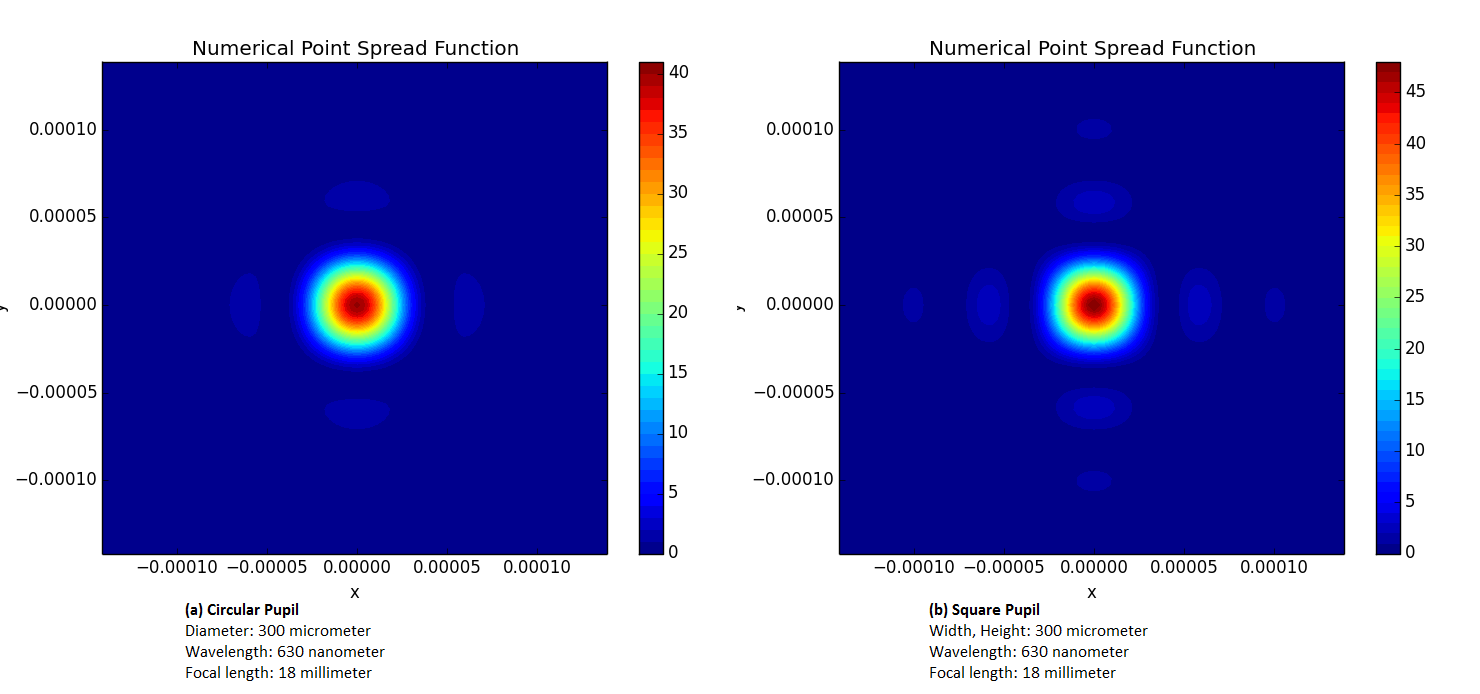
\includegraphics[width=1.0\textwidth]{figures/PupilShape.png}
	\caption{PSF for (a) a circular pupil function of diameter D and (b) a square pupil function of width D. }
	\label{fig:Pupils}
\end{figure}
